\documentclass[12pt]{article}
\usepackage{hyperref}
\usepackage{listings}
\usepackage[margin=1in]{geometry}
\usepackage{enumitem}
\usepackage{multicol}
\usepackage{array}
\usepackage{titlesec}
\usepackage{helvet}
\renewcommand{\familydefault}{\sfdefault}
\usepackage{amsmath}     % For math equations
\usepackage{amssymb}     % For advanced math symbols
\usepackage{amsfonts} % For math fonts
\usepackage{gvv}
\usepackage{esint}
\usepackage[utf8]{inputenc}
\usepackage{graphicx}
\usepackage{pgfplots}
\pgfplotsset{compat=1.18}
\titleformat{\section}{\bfseries\large}{\thesection.}{1em}{}
\setlength{\parindent}{0pt}
\setlength{\parskip}{6pt}
\usepackage{multirow}

\usepackage{fancyhdr}     % For custom headers and footers

\pagestyle{fancy}         % Use the fancy page style
\fancyhf{}                % Clear existing header/footer

% Header customization
\renewcommand{\headrulewidth}{0.4pt}          % Horizontal line at top
\fancyhead[L]{\textbf{2012}}                       % Page number on left
\fancyhead[R]{\textbf{ENGINEERING SCIENCES – XE}}  % Custom text on right
\cfoot{\thepage}

\usepackage[siunitx,RPvoltages]{circuitikz}
\usepackage{tikz}
\usepackage{float}
\usepackage{caption}

\begin{document}

\begin{center}
    {\Large \textbf{XE : ENGINEERING SCIENCES}} \\
    \textit{Duration: Three Hours} \hfill \textbf{Maximum Marks: 100}
\end{center}

\noindent\textbf{Read the following instructions carefully.}

\begin{enumerate}[leftmargin=*]
    \item Do not open the seal of the Question Booklet until you are asked to do so by the invigilator.
    \item Take out the Optical Response Sheet (\textbf{ORS}) from this Question Booklet \textbf{without breaking the seal} and read the instructions printed on the ORS carefully.
    \item On the right half of the ORS, using \textbf{ONLY a black ink ball point pen}, (i) darken the bubble corresponding to your test paper code and the appropriate bubble under each digit of your registration number and (ii) write your registration number, your name and name of the examination centre and put your signature at the specified location.
    \item This Question Booklet contains \textbf{36 pages} including blank pages for rough work. After you are permitted to open the seal, please check all pages and report discrepancies, if any, to the invigilator.
    \item There are a total of \textbf{65 questions} carrying 100 marks. All these questions are of objective type. Each question has only one correct answer. Questions must be answered on the left hand side of the ORS by darkening the appropriate bubble (marked A, B, C, D) using \textbf{ONLY a black ink ball point pen} against the question number. For each question darken the bubble of the correct answer. More than one answer bubbled against a question will be treated as an incorrect response.
    \item Since bubbles darkened by the black ink ball point pen \textbf{cannot be erased}, candidates should darken the bubbles in the ORS \textbf{very carefully}.
    \item This Question Booklet contains \textbf{eight sections}: GA (General Aptitude), A (Engineering Mathematics), B (Fluid Mechanics), C (Materials Science), D (Solid Mechanics), E (Thermodynamics), F (Polymer Science \& Engineering) and G (Food Technology).
    \item Sections GA (General Aptitude) and Section A (Engineering Mathematics) are compulsory. Answer any two optional sections B through G. Using a \textbf{black ink ball point pen}, mark the sections you have chosen by darkening the appropriate bubbles provided on the left hand side of the ORS. Also, write the codes of the optional sections in the boxes provided. In case the candidate \textbf{does not bubble} section codes corresponding to Optional Section-1 or Optional Section-2 or both, the corresponding sections will \textbf{NOT be evaluated}.
    \item Questions Q.1--Q.10 belong to Section GA (General Aptitude) and carry a total of 15 marks. Questions Q.1--Q.5 carry 1 mark each, and questions Q.6--Q.10 carry 2 marks each.
    \item There are 11 questions carrying 15 marks in Section A (Engineering Mathematics), which is compulsory. Questions Q.1--Q.7 carry 1 mark each and questions Q.8--Q.11 carry 2 marks each.
    \item Each of the other sections (Sections B through G) contains 22 questions carrying 35 marks. Questions Q.1--Q.9 carry 1 mark each and questions Q.10--Q.22 carry 2 marks each. The 2 marks questions include two pairs of common data questions and one pair of linked answer questions. The answer to the second question of the linked answer questions depends on the answer to the first question of the pair. If the first question in the linked pair is wrongly answered or is unattempted, then the answer to the second question in the pair will not be evaluated.
    \item Unattempted questions will result in zero mark and wrong answers will result in \textbf{NEGATIVE marks}. For all 1 mark questions, $\tfrac{1}{3}$ mark will be deducted for each wrong answer. For all 2 marks questions, $\tfrac{2}{3}$ mark will be deducted for each wrong answer. However, in the case of the linked answer question pair, there will be negative marks only for wrong answer to the first question and no negative marks for wrong answer to the second question.
    \item Calculator is allowed whereas charts, graph sheets or tables are \textbf{NOT} allowed in the examination hall.
    \item Before the start of the examination, write your name and registration number in the space provided below using a black ink ball point pen.
\end{enumerate}

\noindent\textbf{Name:} \rule{8cm}{0.4pt} \newline \textbf{Registration Number:} \rule{5cm}{0.4pt} \\
\noindent\textbf{XE} 

\newpage

\section*{General Aptitude (GA) Questions (Compulsory)}

\begin{enumerate}

\item[] \textbf{Q.1 - Q.5 carry one mark each.}

\item One of the parts in the sentence given below contains an ERROR.  
Which one of the following is INCORRECT?  

\textbf{I requested that he should be given the driving test today instead of tomorrow.}  

\begin{enumerate}
\item requested that
\item should be given
\item the driving test
\item instead of tomorrow
\end{enumerate}

(GATE XE 2012)

\item Which one of the following options is the closest in meaning to the word given below?  

\textbf{Latitude}  

\begin{multicols}{4}
\begin{enumerate}
\item Eligibility
\item Freedom
\item Coercion
\item Meticulousness
\end{enumerate}
\end{multicols}

(GATE XE 2012)

\item Choose the most appropriate word from the options given below to complete the following sentence:  

Given the seriousness of the situation that he had to face, his \textbf{-----} was impressive.  

\begin{multicols}{4}
\begin{enumerate}
\item beggary
\item nomenclature
\item jealousy
\item nonchalance
\end{enumerate}
\end{multicols}

(GATE XE 2012)

\item Choose the most appropriate alternative from the options given below to complete the following sentence:  

If the tired soldier wanted to lie down, he \textbf{-----} the mattress out on the balcony.  

\begin{enumerate}
\item should take
\item shall take
\item should have taken
\item will have taken
\end{enumerate}

(GATE XE 2012)

\item If $(1.001)^{1259} = 3.52$ and $(1.001)^{2062} = 7.85$, then $(1.001)^{3321} =$  

\begin{multicols}{4}
\begin{enumerate}
\item 2.23
\item 4.33
\item 11.37
\item 27.64
\end{enumerate}
\end{multicols}

(GATE XE 2012)



\item[] \textbf{Q.6 -- Q.10 carry two marks each.}


\item A and B are friends. They decide to meet between 1 PM and 2 PM on a given day.  
There is a condition that whoever arrives first will not wait for the other for more than 15 minutes.  
The probability that they will meet on that day is  

\begin{multicols}{4}
\begin{enumerate}
\item 1/4
\item 1/16
\item 7/16
\item 9/16
\end{enumerate}
\end{multicols}

(GATE XE 2012)

\item The data given in the following table summarizes the monthly budget of an average household.  

\begin{table}[H]
\centering
\caption{}
\label{}
\begin{tabular}{|c|c|}
\hline
\textbf{Category} & \textbf{Amount (Rs.)} \\
\hline
Food & 4000 \\
\hline
Clothing & 1200 \\
\hline
Rent & 2000 \\
\hline
Savings & 1500 \\
\hline
Other expenses & 1800 \\
\hline
\end{tabular}
\end{table}

The approximate percentage of the monthly budget \textbf{NOT spent on savings} is  

\begin{multicols}{4}
\begin{enumerate}
\item 10\%
\item 14\%
\item 81\%
\item 86\%
\end{enumerate}
\end{multicols}

(GATE XE 2012)

\item There are eight bags of rice looking alike, seven of which have equal weight and one is slightly heavier. The weighing balance is of unlimited capacity. Using this balance, the minimum number of weighings required to identify the heavier bag is  

\begin{multicols}{4}
\begin{enumerate}
\item 2
\item 3
\item 4
\item 8
\end{enumerate}
\end{multicols}

(GATE XE 2012)

\item Raju has 14 currency notes in his pocket consisting of only Rs. 20 notes and Rs. 10 notes. The total money value of the notes is Rs. 230. The number of Rs. 10 notes that Raju has is  

\begin{multicols}{4}
\begin{enumerate}
\item 5
\item 6
\item 9
\item 10
\end{enumerate}
\end{multicols}

(GATE XE 2012)

\item \textbf{One of the legacies of the Roman legions was discipline. In the legions, military law prevailed and discipline was brutal. Discipline on the battlefield kept units obedient, intact and fighting, even when the odds and conditions were against them.}  

Which one of the following statements best sums up the meaning of the above passage?  

\begin{enumerate}
\item Thorough regimentation was the main reason for the efficiency of the Roman legions even in adverse circumstances.  
\item The legions were treated inhumanly as if the men were animals.  
\item Discipline was the armies’ inheritance from their seniors.  
\item The harsh discipline to which the legions were subjected to led to the odds and conditions being against them.  
\end{enumerate}

(GATE XE 2012)
\end{enumerate}

\newpage

\begin{center}
{\Large \textbf{A : ENGINEERING MATHEMATICS (Compulsory)}}
\end{center}

\begin{enumerate}

\item[] \textbf{ Q. 1 -- Q. 7 carry one mark each.}

\item For the matrix 
M = \myvec{
1 & 4 & 5 \\ 
0 & 2 & 6 \\ 
0 & 0 & 3}
,
consider the following statements:  

P: 3 is an eigenvalue of $M$.  
Q: \myvec{4 \\ 1 \\ 0}  is an eigenvector of $M$.  
R: \myvec{4 \\ 2 \\ 0}  is an eigenvector of $M$.  

Which of the above statements are TRUE?  

\begin{multicols}{2}
\begin{enumerate}
\item P and Q, but not R  
\item Q and R, but not P  
\item P and R, but not Q  
\item P, Q and R
\end{enumerate}
\end{multicols}

(GATE XE 2012)

\item Taylor series of $f(x) = \dfrac{1}{1-x}$ about $x=0$ is given as  
$
TS|_{x=0} = 1 + x + x^2 + x^3 + \dots
$
This series can be used to evaluate $f(x)$ for  

\begin{multicols}{4}
\begin{enumerate}
\item $|x| \neq 1$  
\item $x < -1$  
\item $|x| < 1$  
\item $-1 \leq x < 1$
\end{enumerate}
\end{multicols}

(GATE XE 2012)

\item Let $f(u,v) = u \ln(v)$ and $F(x,y) = f(u(x,y), v(x,y))$, where $u = x/y$ and $v = x-y$.  
Then $\dfrac{\partial F}{\partial y}$ is  

\begin{multicols}{2}
\begin{enumerate}
\item $-\dfrac{x}{y^2}\ln(x-y) + \dfrac{x}{y(x-y)}$  
\item $-\dfrac{x}{y^2}\ln v - \dfrac{u}{v}$  
\item $\dfrac{x}{y^2}\ln v - \dfrac{u}{v}$  
\item $\dfrac{x}{y^2}\ln v + \dfrac{x}{yv}$
\end{enumerate}
\end{multicols}

(GATE XE 2012)

\item Consider two functions $f(z) = |z|$ and $g(z) = \overline{z}$ (conjugate of $z$).  
Using Cauchy-Riemann conditions, choose the correct answer:  

\begin{multicols}{2}
\begin{enumerate}
\item Both $f$ and $g$ are analytic  
\item $f$ is analytic but $g$ is not analytic  
\item $g$ is analytic but $f$ is not analytic  
\item Neither $f$ nor $g$ is analytic
\end{enumerate}
\end{multicols}

(GATE XE 2012)

\item For $f(x,y) = x^4 - 5xy^2$, the direction of maximum increase of $f(x,y)$ at the point $(2,2)$ is along  

\begin{multicols}{4}
\begin{enumerate}
\item $3\hat{i} + 10\hat{j}$  
\item $-12\hat{i} - 40\hat{j}$  
\item $3\hat{i} - 10\hat{j}$  
\item $-12\hat{i} + 40\hat{j}$
\end{enumerate}
\end{multicols}

(GATE XE 2012)

\item Suppose 50\% of the population of a village like oranges, 70\% of the population like apples, and 40\% like both.  
If a person is picked at random who likes at least one of these fruits, what is the probability that the person likes oranges?  

\begin{multicols}{4}
\begin{enumerate}
\item $1/8$  
\item $5/12$  
\item $1/2$  
\item $5/8$
\end{enumerate}
\end{multicols}

(GATE XE 2012)

\item For the solution of $\nabla^{2}u = 0$, the domain and boundary conditions are shown below.

\begin{figure}[H]
    \centering
    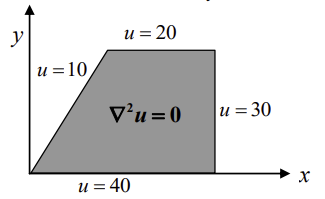
\includegraphics[width=0.5\columnwidth]{figs/ass2_a_q7.png}
    \caption{}
    \label{fig:placeholder}
\end{figure}
Which of the following statements is \textbf{TRUE}?
\begin{enumerate}
\item The solution cannot be obtained using separation of variables because the governing equation is non-separable.
\item The solution cannot be obtained using separation of variables because all the boundary values are non-zero.
\item The solution cannot be obtained using separation of variables because not all the boundaries are along constant coordinate lines.
\item The solution can be obtained by separation of variables.
\end{enumerate}

(GATE XE 2012)

\item[] \textbf{Q.8 - Q.11 carry two marks each.}

\item If $f(x) = x\sin(x)$ and $g(x) = |x|\sin(x)$, then
\begin{enumerate}
\item $g(x) = |f(x)|$
\item $g(x)$ is an even function
\item The $x$-coordinates corresponding to the various local maxima are identical for both $f(x)$ and $g(x)$
\item $g(x)$ is differentiable at $x=0$
\end{enumerate}

(GATE XE 2012)

\item The general solution of $\dfrac{d^{4}y}{dx^{4}} - 2\dfrac{d^{3}y}{dx^{3}} + 2\dfrac{d^{2}y}{dx^{2}} - 2\dfrac{dy}{dx} + y = 0$ is
\begin{enumerate}
\item $c_{1}e^{x} + c_{2}xe^{x} + c_{3}\cosh(x) + c_{4}\sinh(x)$
\item $c_{1}e^{x} + c_{2}e^{-x} + c_{3}e^{ix} + c_{4}e^{-ix}$
\item $c_{1}e^{x} + c_{2}xe^{x} + c_{3}\cos(x) + c_{4}\sin(x)$
\item $c_{1}e^{x} + c_{2}xe^{-x} + c_{3}e^{ix} + c_{4}e^{-ix}$
\end{enumerate}

(GATE XE 2012)

\item Evaluation of $\iint_{S}(e^{x}\hat{i} + 3y\hat{j} - ze^{z}\hat{k}) \cdot \hat{n} \, dA$ over a surface $S: x^{2}+y^{2}+z^{2}=1$, using Gauss divergence theorem, gives
\begin{multicols}{2}
\begin{enumerate}
\item 0
\item $4\pi$
\item $\dfrac{4\pi}{3}$
\item $12\pi$
\end{enumerate}
\end{multicols}

(GATE XE 2012)

\item The exact solution of the integral $\int_{0}^{4}(x^{2}-4)\,dx$ is denoted by $I_{E}$. The same integral evaluated numerically by the trapezoidal rule and the Simpson’s 1/3 rule are denoted by $I_{T}$ and $I_{S}$, respectively. The subinterval used in the numerical methods is $h=2$. Then
\begin{multicols}{2}
\begin{enumerate}
\item $I_{E} = I_{S} > I_{T}$
\item $I_{E} = I_{S} < I_{T}$
\item $I_{E} < I_{S} < I_{T}$
\item $I_{E} > I_{S} > I_{T}$
\end{enumerate}
\end{multicols}

(GATE XE 2012)

\end{enumerate}

\begin{center}
\textbf{END OF SECTION - A}
\end{center}

\newpage

\begin{center}
{\Large \textbf{B : FLUID MECHANICS}}
\end{center}

\begin{enumerate}

\item[] \textbf{Q.1 -- Q.9 carry one mark each.}


\item In a two-dimensional flow field, the velocities in the $x$- and $y$- directions are $u$ and $v$, respectively. The shear stress for a Newtonian fluid having dynamic viscosity $\mu$ is given by
\begin{multicols}{4}
\begin{enumerate}
\item $\mu \left( \dfrac{\partial v}{\partial x} + \dfrac{\partial u}{\partial y} \right)$
\item $2\mu \dfrac{\partial v}{\partial y}$
\item $2\mu \dfrac{\partial u}{\partial x}$
\item $\mu \left( \dfrac{\partial v}{\partial x} - \dfrac{\partial u}{\partial y} \right)$
\end{enumerate}
\end{multicols}

(GATE XE 2012)

\item In a potential flow, the superposition of the stream functions of a uniform flow and a line source gives rise to a dividing streamline representing
\begin{multicols}{2}
\begin{enumerate}
\item Rankine’s half-body
\item infinite circular cylinder
\item infinite rotating circular cylinder
\item infinite elliptical cylinder
\end{enumerate}
\end{multicols}

(GATE XE 2012)

\item Given that $V$, $L$ and $g$ are the characteristic velocity, characteristic length and acceleration due to gravity, respectively, the expression $\dfrac{V}{\sqrt{Lg}}$ represents
\begin{multicols}{4}
\begin{enumerate}
\item Weber number
\item Euler number
\item Cavitation number
\item Froude number
\end{enumerate}
\end{multicols}

(GATE XE 2012)

\item Match the devices in Column I with the characteristics in Column II.

\begin{center}
\begin{table}[H]
\centering \caption{} \label{}
\begin{tabular}{l l}
\textbf{Column I} & \textbf{Column II} \\
P. orifice meter & 1. high head loss and low cost \\
Q. venturi meter & 2. high head loss and high cost \\
& 3. low head loss and high cost \\
& 4. low head loss and low cost \\
\end{tabular}
\end{table}
\end{center}

\begin{multicols}{4}
\begin{enumerate}
\item P = 2 ; Q = 4
\item P = 1 ; Q = 2
\item P = 3 ; Q = 1
\item P = 1 ; Q = 3
\end{enumerate}
\end{multicols}

(GATE XE 2012)

\item Identify the visualization method that shows a PATHLINE in an unsteady flow, assuming that the camera covers the required field of view.
\begin{enumerate}
\item A dye is continuously injected and a snap shot is taken
\item A dye is continuously injected and a long-exposure picture is taken
\item A blob (or drop) of dye is injected and a snap shot is taken
\item A blob (or drop) of dye is injected and a long-exposure picture is taken
\end{enumerate}

(GATE XE 2012)

\item In the case of a fully developed flow through a pipe, the shear stress at the centerline is
\begin{multicols}{2}
\begin{enumerate}
\item a function of the axial distance
\item a function of the centerline velocity
\item zero
\item infinite
\end{enumerate}
\end{multicols}

(GATE XE 2012)

\item The velocity in a one-dimensional unsteady flow is given by $(x^{2} - t)$, where $x$ is the position and $t$ is the time. The total acceleration at any $x$ and $t$ is
\begin{multicols}{4}
\begin{enumerate}
\item $-1 + x t + x^{3}$
\item $-1 + x t + 2x^{3}$
\item $-1 - x t - x^{3}$
\item $-1 - 2x t + 2x^{3}$
\end{enumerate}
\end{multicols}

(GATE XE 2012)

\item If $\psi$ is the stream function, the Laplace’s equation $\nabla^{2}\psi = 0$ is true when the flow is
\begin{multicols}{2}
\begin{enumerate}
\item incompressible
\item incompressible and irrotational
\item irrotational
\item compressible
\end{enumerate}
\end{multicols}

(GATE XE 2012)

\item A fully developed laminar flow is taking place through a pipe. If the flow velocity is doubled maintaining the flow laminar, the pressure loss would be
\begin{multicols}{4}
\begin{enumerate}
\item halved
\item unaltered
\item doubled
\item trebled
\end{enumerate}
\end{multicols}

(GATE XE 2012)

\item[] \textbf{Q.10-Q.22 carry two marks each.}

\item In the following equations, $u$ and $v$ are the velocities in the $x$- and $y$- directions, respectively and $t$ is time. The flow field that CANNOT be termed as incompressible is

\begin{multicols}{2}
\begin{enumerate}
\item $u = x^{3} + x y^{2}, \; v = y^{3} + y x^{2}$
\item $u = 10xt, \; v = -10yt$
\item $u = \left(\dfrac{y}{\delta}\right)^{1/7}, \; v = 0 \;\; (\delta = \text{constant})$
\item $u = 2y, \; v = 2x$
\end{enumerate}
\end{multicols}

(GATE XE 2012)

\item A U-tube mercury (Hg) manometer as shown below is employed to measure the pressure of an oil-filled vessel. The densities of Hg and oil are $13600 \; \text{kg/m}^{3}$ and $800 \; \text{kg/m}^{3}$, respectively. The gravitational acceleration may be taken as $10 \; \text{m/s}^{2}$. The gauge pressure (in Pa) at point A when $h_{1} = 0.5 \; \text{m}$ and $h_{2} = 0.9 \; \text{m}$, is approximately

\begin{figure}[H]
    \centering
    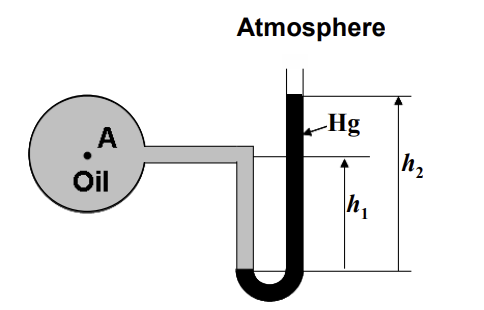
\includegraphics[width=0.5\columnwidth]{figs/ass2_b_q11.png}
    \caption{}
    \label{fig:placeholder}
\end{figure}

\begin{multicols}{4}
\begin{enumerate}
\item $118.4 \times 10^{3}$
\item $118.4$
\item $11.84$
\item $1.184$
\end{enumerate}
\end{multicols}

(GATE XE 2012)

\item Water is supplied to a tank at the rate of $0.02 \; \text{m}^{3}/\text{s}$, as shown in the figure below. The cross-sectional area of the tank is $1 \; \text{m}^{2}$ and the inner diameter of the outlet pipe is $60 \; \text{mm}$. At a time when the water level in the tank is increasing at the rate of $5 \; \text{mm/s}$, the average velocity (in m/s) of water in the outlet pipe is approximately

\begin{figure}[H]
    \centering
    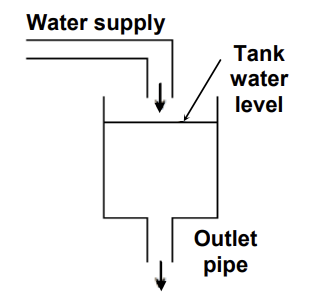
\includegraphics[width=0.5\columnwidth]{figs/ass2_b_q12.png}
    \caption{}
    \label{fig:placeholder}
\end{figure}

\begin{multicols}{4}
\begin{enumerate}
\item 0.005
\item 0.06
\item 5.3
\item 20
\end{enumerate}
\end{multicols}

(GATE XE 2012)

\item The water level in the tank is $4.2 \, \text{m}$ above the pipe centerline as indicated. The gas pressure is $130 \, \text{kPa}$. The atmospheric pressure, gravitational acceleration and density of water may be taken as $100 \, \text{kPa}, \; 10 \, \text{m/s}^{2}$ and $1000 \, \text{kg/m}^{3}$, respectively. Neglecting losses, the maximum velocity (in m/s) of water at any location in the horizontal portion of the delivery pipe for the pressure NOT to drop below atmospheric pressure, is

\begin{figure}[H]
    \centering
    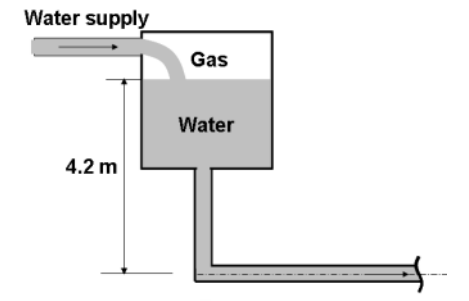
\includegraphics[width=0.5\columnwidth]{figs/ass2_b_q13.png}
    \caption{}
    \label{fig:placeholder}
\end{figure}
\begin{multicols}{4}
\begin{enumerate}
\item 1.3
\item 4.2
\item 10
\item 12
\end{enumerate}
\end{multicols}

(GATE XE 2012)

\item The figure given below shows typical non-dimensional velocity profiles for fully developed laminar flow between two infinitely long parallel plates separated by a distance $a$ along $y$-direction. The upper plate is moving with a constant velocity $U$ in the $x$-direction and the lower plate is stationary.  

\begin{figure}[H]
    \centering
    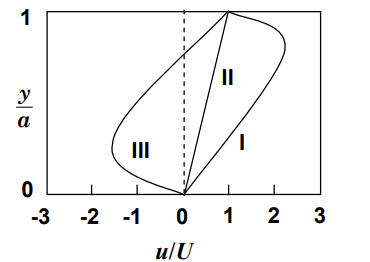
\includegraphics[width=0.5\columnwidth]{figs/ass2_b_q14.png}
    \caption{}
    \label{fig:placeholder}
\end{figure}

Match the non-dimensional velocity profiles in Column I with the pressure gradients in Column II.

\begin{center}
\begin{table}[H]
\centering
\caption{} \label{}
\begin{tabular}{l l}

\textbf{Column I} & \textbf{Column II} \\
P. profile I & 1. $\dfrac{\partial p}{\partial x} > 0$ \\
Q. profile II & 2. $\dfrac{\partial p}{\partial x} < 0$ \\
R. profile III & 3. $\dfrac{\partial p}{\partial x} = 0$ \\
\end{tabular}
\end{table}
\end{center}

\begin{multicols}{2}
\begin{enumerate}
\item P = 2 ; Q = 3 ; R = 1
\item P = 3 ; Q = 2 ; R = 1
\item P = 3 ; Q = 1 ; R = 2
\item P = 1 ; Q = 2 ; R = 3
\end{enumerate}
\end{multicols}

(GATE XE 2012)

\item Air flows over a spherical storage vessel of diameter $4 \, \text{m}$ at a speed of $1 \, \text{m/s}$. To find the drag force on the vessel, a test run is to be carried out in water using a sphere of diameter $100 \, \text{mm}$. The density and dynamic viscosity of air are $1.2 \, \text{kg/m}^{3}$ and $1.8 \times 10^{-5} \, \text{Pa.s}$, respectively. The density and dynamic viscosity of water are $1000 \, \text{kg/m}^{3}$ and $10^{-3} \, \text{Pa.s}$, respectively. The drag force on the model is $4 \, \text{N}$ under dynamically similar conditions. The drag force (in N) on the prototype is approximately
\begin{multicols}{4}
\begin{enumerate}
\item 0.25
\item 0.93
\item 1.08
\item 4
\end{enumerate}
\end{multicols}

(GATE XE 2012)

\item The velocity of an air stream is $20 \, \text{m/s}$. The densities of mercury and air are $13600 \, \text{kg/m}^{3}$ and $1.2 \, \text{kg/m}^{3}$, respectively. The gravitational acceleration may be taken as $10 \, \text{m/s}^{2}$. When a Pitot-static tube is placed in the stream, assuming the flow to be incompressible and frictionless, the difference between the stagnation and static pressure in the flow field (in mm Hg) would approximately be
\begin{multicols}{4}
\begin{enumerate}
\item $1760$
\item $1.76$
\item $0.57$
\item $0.57 \times 10^{-5}$
\end{enumerate}
\end{multicols}

(GATE XE 2012)



\item[] {\large\textbf{Common Data Questions} }

\textbf{Common Data for Questions 17 and 18:}  

A vessel containing water (density $1000 \, \text{kg/m}^{3}$) and oil (density $800 \, \text{kg/m}^{3}$), pressurized by gas, is shown. Assume that the gravitational acceleration is $10 \, \text{m/s}^{2}$.  

\begin{figure}[H]
    \centering
    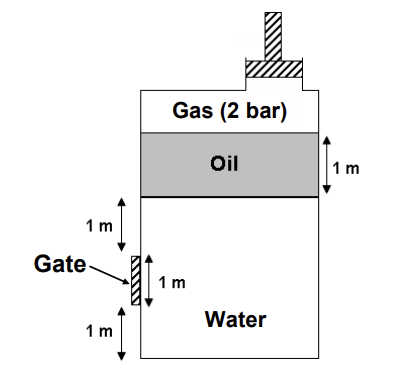
\includegraphics[width=0.5\columnwidth]{figs/ass2_b_q16.png}
    \caption{}
    \label{fig:placeholder}
\end{figure}

\item The pressure (in bar) exerted on the bottom wall inside the vessel is approximately
\begin{multicols}{4}
\begin{enumerate}
\item 0.238
\item 2.38
\item 23.8
\item 238
\end{enumerate}
\end{multicols}

(GATE XE 2012)

\item The gate is $1 \, \text{m}$ wide perpendicular to the plane of the paper. The force (in N) exerted on the gate is approximately
\begin{multicols}{4}
\begin{enumerate}
\item $2.23 \times 10^{3}$
\item $2.23 \times 10^{4}$
\item $2.23 \times 10^{5}$
\item $2.23 \times 10^{6}$
\end{enumerate}
\end{multicols}

(GATE XE 2012)

\item[] \textbf{Common Data for Questions 19 and 20:}

A boat is propelled in still water at a velocity of $5 \,\text{m/s}$ by taking water at the rate of $1 \,\text{m}^3/\text{s}$ from the aft side and discharging it through the stern using a pump, as shown in the figure below. The velocity of the discharge jet relative to the boat is $9 \,\text{m/s}$. The effect of pressure at the intake and discharge can be neglected. The density of water may be taken as $1000 \,\text{kg/m}^3$.

\begin{figure}[H]
    \centering
    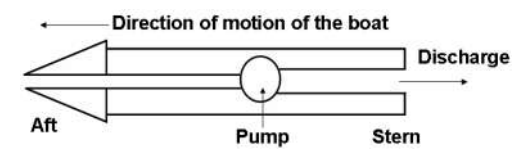
\includegraphics[width=0.5\columnwidth]{figs/ass2_b_q19.png}
    \caption{Caption}
    \label{fig:placeholder}
\end{figure}

\item The power (in kW) required to propel the boat is
\begin{multicols}{4}
\begin{enumerate}
\item 10
\item 20
\item 50
\item 90
\end{enumerate}
\end{multicols}

(GATE XE 2012)

\item The total kinetic energy imparted to the water per second (in kW) by the pump is
\begin{multicols}{4}
\begin{enumerate}
\item 10
\item 25
\item 28
\item 81
\end{enumerate}
\end{multicols}

(GATE XE 2012)

\item[] {\large \textbf{Linked Answer Questions}}

\textbf{Statement for Linked Answer Questions 21 and 22:}

The hydrodynamic boundary layer over a flat plate is shown in the figure below. The velocity in the $x$-direction is approximated as $u = a + by + cy^2$, where $a$, $b$ and $c$ are constants. $U$ is the free stream velocity and $\delta$ is the boundary-layer thickness at any point $x$ on the plate.

\begin{figure}[H]
    \centering
    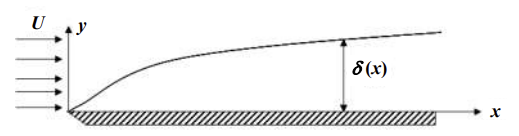
\includegraphics[width=0.5\columnwidth]{figs/ass2_b_q21.png}
    \caption{Caption}
    \label{fig:placeholder}
\end{figure}

\item The dimensionless velocity profile is
\begin{multicols}{2}
\begin{enumerate}
\item $\dfrac{u}{U} = 2\left(\dfrac{y}{\delta}\right) - \left(\dfrac{y}{\delta}\right)^2$
\item $\dfrac{u}{U} = 2\left(\dfrac{y}{\delta}\right) + \left(\dfrac{y}{\delta}\right)^2$
\item $\dfrac{u}{U} = 1.5\left(\dfrac{y}{\delta}\right) - 0.5\left(\dfrac{y}{\delta}\right)^2$
\item $\dfrac{u}{U} = 1.5\left(\dfrac{y}{\delta}\right) + 0.5\left(\dfrac{y}{\delta}\right)^2$
\end{enumerate}
\end{multicols}

(GATE XE 2012)

\item The displacement thickness (in mm) when $\delta = 6 \,\text{mm}$, is
\begin{multicols}{4}
\begin{enumerate}
\item 2.25
\item 2
\item -2
\item -2.25
\end{enumerate}
\end{multicols}

(GATE XE 2012)

\end{enumerate}

\begin{center}
\textbf{END OF SECTION - B}
\end{center}

\newpage

\begin{center}
{\Large \textbf{C : MATERIALS SCIENCE}}
\end{center}

\begin{table}[H]
\centering
\begin{tabular}{>{\bfseries}l l}
Useful data &  \\
Boltzmann’s constant & $1.38 \times 10^{-23}\,\text{J K}^{-1}$ \\
Charge on an electron & $1.602 \times 10^{-19}\,\text{C}$ \\
Gas Constant & $8.314 \,\text{J mol}^{-1}\,\text{K}^{-1}$ \\
Electron rest mass & $9.1 \times 10^{-31}\,\text{kg}$ \\
Permittivity of vacuum ($\varepsilon_0$) & $8.854 \times 10^{-12}\,\text{F m}^{-1}$ \\
Bohr Magneton & $9.274 \times 10^{-24}\,\text{A m}^2$ \\
\end{tabular}
\caption{}
\label{}
\end{table}

\begin{enumerate}
\item[] \textbf{Q.1 – Q.9 carry one mark each.}

\item Which of the following is NOT a Bravais lattice?
\begin{enumerate}
\item Simple tetragonal
\item Body centered tetragonal
\item Base centred orthorhombic
\item Face centred tetragonal
\end{enumerate}
(GATE XE 2012)

\item A Schottky defect in an ionic crystal is a stoichiometric defect of
\begin{enumerate}
\item Cation vacancy
\item Anion vacancy
\item Cation and anion vacancy
\item Cation and anion interstitial
\end{enumerate}
(GATE XE 2012)

\item Which of the following techniques is NOT used to grow single crystals of semiconductors?
\begin{multicols}{4}
\begin{enumerate}
\item Calendering
\item Czochralski
\item Float zone
\item Bridgman
\end{enumerate}
\end{multicols}
(GATE XE 2012)

\item Which of the following signals is produced due to the elastic scattering of electrons by a material?
\begin{enumerate}
\item Secondary electron
\item Backscattered electron
\item Auger electron
\item Photoelectron
\end{enumerate}
(GATE XE 2012)

\item The best magnetostrictive material is
\begin{multicols}{4}
\begin{enumerate}
\item Nd$_2$Fe$_{14}$B
\item Fe$_3$O$_4$
\item Cu$_2$MnAl
\item ZnFe$_2$O$_4$
\end{enumerate}
\end{multicols}
(GATE XE 2012)

\item Of the following materials, which is the most suitable for an LED emitting at around 380 nm?
\begin{enumerate}
\item Direct bandgap material with a small bandgap
\item Indirect bandgap material with a large bandgap
\item Direct bandgap material with a large bandgap
\item Indirect bandgap material with a small bandgap
\end{enumerate}
(GATE XE 2012)

\item Which material has the lowest specific heat capacity at room temperature?
\begin{multicols}{4}
\begin{enumerate}
\item Water
\item Mercury
\item Copper
\item Silver
\end{enumerate}
\end{multicols}
(GATE XE 2012)

\item Microstrain can be measured by X-ray diffraction using peak
\begin{enumerate}
\item Area and intensity
\item Position and area
\item Broadening and intensity
\item Position and broadening
\end{enumerate}
(GATE XE 2012)


\item The Pilling-Bedworth ratio is defined as the ratio of
\begin{enumerate}
\item Volume of oxide to volume of metal
\item Weight of oxide to weight of metal
\item Density of oxide to density of metal
\item Surface area of oxide to surface area of metal
\end{enumerate}
(GATE XE 2012)

\item[]  \textbf{Q.10-Q.22 carry two marks each.}

\item Match the properties in Column I with the appropriate units in Column II

\begin{table}[h]
\centering
\begin{tabular}{l l}
\textbf{Column I} & \textbf{Column II} \\
P. Thermal diffusivity & 1. Hm$^{-1}$ \\
Q. Fracture toughness & 2. m$^{2}$s$^{-1}$ \\
R. Surface energy & 3. Fm$^{-1}$ \\
S. Magnetic permeability & 4. Nm$^{-3/2}$ \\
& 5. Jm$^{-2}$ \\
\end{tabular}
\caption{}
\label{}
\end{table}

\begin{multicols}{2}
\begin{enumerate}
\item P-2, Q-5, R-4, S-1
\item P-2, Q-4, R-5, S-1
\item P-3, Q-5, R-4, S-3
\item P-5, Q-4, R-2, S-3
\end{enumerate}
\end{multicols}
(GATE XE 2012)

\item Match the characterization techniques in Column I with the options in Column II

\begin{table}[h]
\centering
\begin{tabular}{l l}
\textbf{Column I} & \textbf{Column II} \\
P. Scanning tunneling microscopy & 1. No vacuum required \\
Q. Scanning electron microscopy & 2. Backscattered electrons \\
R. Transmission electron microscopy & 3. Photoelectrons \\
S. Atomic force microscopy & 4. Atomically sharp tip \\
& 5. Sub-Angstrom resolution \\
\end{tabular}
\caption{}
\label{}
\end{table}

\begin{multicols}{2}
\begin{enumerate}
\item P-4, Q-2, R-5, S-1
\item P-1, Q-3, R-4, S-5
\item P-2, Q-4, R-1, S-5
\item P-5, Q-1, R-2, S-4
\end{enumerate}
\end{multicols}
(GATE XE 2012)

\item Match the materials in Column I with the applications in Column II

\begin{table}[h]
\centering
\begin{tabular}{l l}
\textbf{Column I} & \textbf{Column II} \\
P. Titanium diboride & 1. Photocatalyst \\
Q. Molybdenum disilicide & 2. Furnace heating element \\
R. Hydroxyapatite & 3. Ultra high temperature material \\
S. Nanocrystalline titanium oxide & 4. Tough ceramic \\
& 5. Artificial bone implant \\
\end{tabular}
\caption{}
\label{}
\end{table}

\begin{multicols}{2}
\begin{enumerate}
\item P-3, Q-4, R-5, S-1
\item P-5, Q-3, R-2, S-1
\item P-4, Q-3, R-1, S-5
\item P-3, Q-2, R-5, S-4
\end{enumerate}
\end{multicols}
(GATE XE 2012)

\item Match the properties in Column I with the options in Column II

\begin{table}[h]
\centering
\begin{tabular}{l l}
\textbf{Column I} & \textbf{Column II} \\
P. Toughness & 1. Resistance to plastic deformation \\
Q. Resilience & 2. Time dependent permanent deformation under constant load \\
R. Creep & 3. Total elongation at failure \\
S. Hardness & 4. Area under the stress-strain curve \\
& 5. Area under the elastic part of the stress-strain curve \\
\end{tabular}
\caption{}
\label{}
\end{table}

\begin{multicols}{2}
\begin{enumerate}
\item P-5, Q-1, R-3, S-2
\item P-4, Q-3, R-2, S-1
\item P-4, Q-5, R-2, S-1
\item P-5, Q-4, R-3, S-2
\end{enumerate}
\end{multicols}
(GATE XE 2012)

 \item Determine the mole fraction of vinyl chloride in a copolymer of vinyl chloride (CH$_2$CHCl) and vinyl acetate (CH$_2$CH-OCOCH$_3$) having molecular weight of 10520 g/mol and degree of polymerization of 160.
  \begin{multicols}{4}
    \begin{enumerate}
      \item 0.14
      \item 0.30
      \item 0.70
      \item 0.86
    \end{enumerate}
  \end{multicols}
  (GATE XE 2012)

  \item The electron concentration in an n-type semiconductor is $5 \times 10^{18}$/m$^3$. If the drift velocity of electrons is 100 m/s in an electric field of 500 V/m, calculate the conductivity of the semiconductor.
  \begin{multicols}{4}
    \begin{enumerate}
      \item 0.16 $\times 10^{-1}$ S/m
      \item 1.60 $\times 10^{-1}$ S/m
      \item 2.50 $\times 10^{-1}$ S/m
      \item 30.05 $\times 10^{-1}$ S/m
    \end{enumerate}
  \end{multicols}
  (GATE XE 2012)

  \item Calculate the saturation magnetization ($M_{sat}$) for bcc iron of lattice parameter 2.866 \AA.
  \begin{multicols}{4}
    \begin{enumerate}
      \item 0.79 $\times 10^6$ A/m
      \item 1.5 $\times 10^6$ A/m
      \item 3.15 $\times 10^6$ A/m
      \item 4.73 $\times 10^6$ A/m
    \end{enumerate}
  \end{multicols}
  (GATE XE 2012)

  \item[] {\large \textbf{Common Data Questions}} 
  
  \textbf{Common Data for Questions 17 and 18:}
  
  A plain 0.45 wt.\% carbon steel is cooled slowly from 900$^\circ$C to just below the eutectoid temperature (723$^\circ$C) so that the following reaction occurs: \\
  $\gamma$ (0.8 wt.\% C) $\leftrightarrow$ $\alpha$ (0.02 wt.\% C) + Fe$_3$C (6.67 wt.\% C).

  \item During cooling from 900$^\circ$C to 723$^\circ$C, the proeutectoid $\alpha$ forms from $\gamma$. Find the volume \% of proeutectoid $\alpha$ just below 723$^\circ$C for the steel.
  \begin{multicols}{4}
    \begin{enumerate}
      \item 44.9\%
      \item 66.1\%
      \item 55.1\%
      \item 34.9\%
    \end{enumerate}
  \end{multicols}
  (GATE XE 2012)

  \item Find the volume \% of pearlite for the steel just below 723$^\circ$C for 0.45 wt.\% carbon steel.
  \begin{multicols}{4}
    \begin{enumerate}
      \item 44.9\%
      \item 55.1\%
      \item 40.9\%
      \item 59.1\%
    \end{enumerate}
  \end{multicols}
  (GATE XE 2012)

  \item[] \textbf{Common Data for Questions 19 and 20:} 
  
  A 20 kN tensile load is applied axially to a steel bar of cross-sectional area 8 cm$^2$ and 1m length. The Young’s modulus of steel ($E_{steel}$) is 200 GPa, and of aluminium ($E_{Al}$) is 70 GPa. The Poisson’s ratio ($\nu$) can be taken as 0.3.

  \item When the same load is applied to an aluminium bar, it is found to give same elastic strain as the steel. Calculate the cross-sectional area of the aluminium bar.
  \begin{multicols}{4}
    \begin{enumerate}
      \item 11.43 cm$^2$
      \item 14.93 cm$^2$
      \item 18.26 cm$^2$
      \item 22.86 cm$^2$
    \end{enumerate}
  \end{multicols}
  (GATE XE 2012)

  \item Calculate the final area of the steel bar after the deformation under the applied load of 20 kN.
  \begin{multicols}{4}
    \begin{enumerate}
      \item 7.9 cm$^2$
      \item 9.7 cm$^2$
      \item 7.0 cm$^2$
      \item 8.1 cm$^2$
    \end{enumerate}
  \end{multicols}
  (GATE XE 2012)

  \item[] {\large \textbf{Linked Answer Questions}} 
  
  \textbf{Statement for Linked Answer Questions 21 and 22:} Chromium has the bcc structure with atomic diameter of 2.494 \AA.

  \item Calculate the lattice parameter of chromium assuming tight atomic bonding.
  \begin{multicols}{4}
    \begin{enumerate}
      \item 1.442 \AA
      \item 2.880 \AA
      \item 4.323 \AA
      \item 5.764 \AA
    \end{enumerate}
  \end{multicols}
  (GATE XE 2012)

  \item Find the first diffraction peak position (2$\theta$) for Cu K$\alpha$ radiation with a wavelength of 1.54 \AA.
  \begin{multicols}{4}
    \begin{enumerate}
      \item 21.76$^\circ$
      \item 33.05$^\circ$
      \item 44.43$^\circ$
      \item 66.10$^\circ$
    \end{enumerate}
  \end{multicols}
  (GATE XE 2012)

\end{enumerate}
\begin{center}
\textbf{END OF SECTION - C}
\end{center}

\newpage

\begin{center}
{\Large\textbf{D : SOLID MECHANICS}}
\end{center}

\begin{enumerate}

\item[] \textbf{Q.1-Q.9 carry one mark each.}

\item The axial force diagram for the weightless beam subjected to the inclined force $P = 5 \, \text{kN}$ is

\begin{figure}[H]
    \centering
    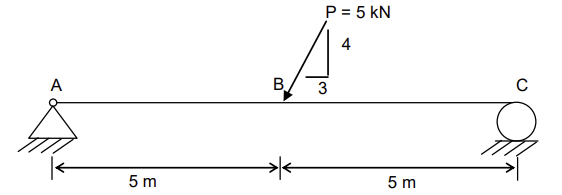
\includegraphics[width=0.5\columnwidth]{figs/ass2_d_q1_q.png}
    \caption{}
    \label{fig:placeholder}
\end{figure}
\begin{enumerate}
\item \begin{figure}[H]
    \centering
    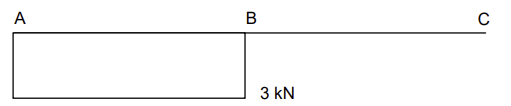
\includegraphics[width=0.5\columnwidth]{figs/ass2_d_q1_a.png}
    \caption{Caption}
    \label{fig:placeholder}
\end{figure}
\item \begin{figure}[H]
    \centering
    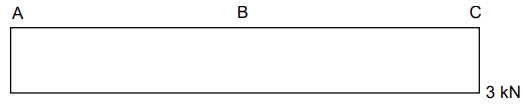
\includegraphics[width=0.5\columnwidth]{figs/ass2_d_q1_b.png}
    \caption{Caption}
    \label{fig:placeholder}
\end{figure}
\item \begin{figure}[H]
    \centering
    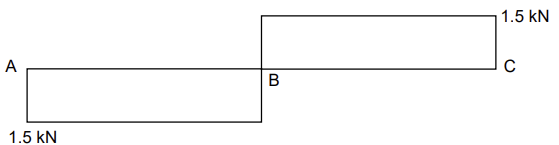
\includegraphics[width=0.5\columnwidth]{figs/ass2_d_q1_c.png}
    \caption{Caption}
    \label{fig:placeholder}
\end{figure}
\item \begin{figure}[H]
    \centering
    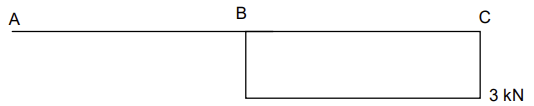
\includegraphics[width=0.5\columnwidth]{figs/ass2_d_q1_d.png}
    \caption{Caption}
    \label{fig:placeholder}
\end{figure}
\end{enumerate}
(GATE XE 2012)

\item A block of weight $W$, connected to two springs with spring constants $k_1$ and $k_2$, rests initially on a horizontal frictional surface. The coefficient of static friction between the block and the surface is $\mu$. Both springs are initially undeformed. The magnitude of force $F$, applied to the second spring, is now gradually increased. The block will start to slide when $F$ becomes

\begin{figure}[H]
    \centering
    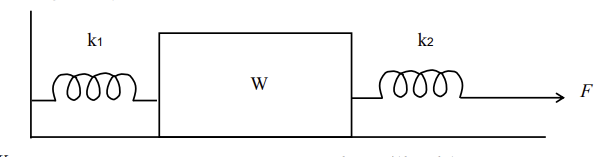
\includegraphics[width=0.5\columnwidth]{figs/ass2_d_q2.png}
    \caption{Caption}
    \label{fig:placeholder}
\end{figure}

\begin{multicols}{2}
\begin{enumerate}
\item $\mu W$
\item $\dfrac{k_1 \mu W}{k_1 + k_2}$
\item $\dfrac{k_2 \mu W}{k_1 + k_2}$
\item $\dfrac{k_2 \mu W}{k_1}$
\end{enumerate}
\end{multicols}
(GATE XE 2012)

\item Three connected railway coaches A, B and C of masses $m_A$, $m_B$ and $m_C$, respectively are being 
pulled by a locomotive with force $F$ over a horizontal track. The coaches may be assumed to move on frictionless wheels with negligible air resistance. The tension in the connector between coaches A and B is  

\begin{figure}[H]
    \centering
    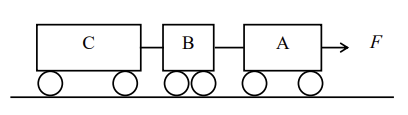
\includegraphics[width=0.5\columnwidth]{figs/ass2_d_q3.png}
    \caption{}
    \label{fig:placeholder}
\end{figure}

\begin{multicols}{2}
\begin{enumerate}
    \item $F$
    \item $\dfrac{F m_A}{m_A+m_B+m_C}$
    \item $\dfrac{F m_B}{m_A+m_B+m_C}$
    \item $\dfrac{F(m_B+m_C)}{m_A+m_B+m_C}$
\end{enumerate}
\end{multicols}
(GATE XE 2012)


\item For the beam-column configurations shown in figure, the minimum Euler buckling load is obtained for the case (Young’s modulus and second moment of cross-sectional area are as indicated)  

\begin{figure}[H]
    \centering
    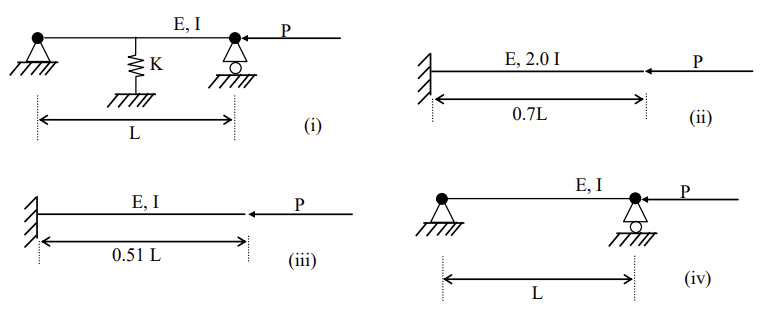
\includegraphics[width=1\columnwidth]{figs/ass2_d_q4.png}
    \caption{}
    \label{fig:placeholder}
\end{figure}

\begin{multicols}{4}
\begin{enumerate}
    \item (i)
    \item (ii)
    \item (iii)
    \item (iv)
\end{enumerate}
\end{multicols}
(GATE XE 2012)


\item A disk of mass $m=0.25~\text{g}$ and radius $r=10~\text{mm}$ is at rest relative to a mass-less horizontal turntable spinning about a vertical axis at an angular speed of $\omega=2~\text{rad/s}$. The turntable is assumed to be mounted on frictionless bearings. Another identical, initially non-rotating disk is dropped onto the spinning disk. Friction causes both disks (and the turntable) to eventually rotate at the same angular speed. The eventual angular speed of the disks is  

\begin{multicols}{4}
\begin{enumerate}
    \item 0.15 rad/s
    \item 1 rad/s
    \item 2 rad/s
    \item 4 rad/s
\end{enumerate}
\end{multicols}
(GATE XE 2012)


\item A rocket in the atmosphere is accelerating upwards with acceleration $a~\text{m/s}^2$. The natural frequency of a spring–mass system (with mass $m$ kg and spring constant $k$ N/m), suspended vertically inside the rocket, is (take $g~\text{m/s}^2$ to be the acceleration due to gravity)  

\begin{multicols}{4}
\begin{enumerate}
    \item $\sqrt{\dfrac{\bar{k}}{m}} \quad (\,\bar{k} < k\,)$
    \item $\sqrt{\dfrac{k}{m}}$
    \item $\sqrt{\dfrac{kg}{ma}}$
    \item $\sqrt{\dfrac{k}{m}\left(1-\tfrac{a}{g}\right)}$
\end{enumerate}
\end{multicols}
(GATE XE 2012)

\item An irregular planar body in space is acted upon by a force $\bar{F} = (2\hat{i} + \hat{j})N$ at position 
$\bar{r}_1 = (\hat{i} + 2\hat{j})m$ and a moment $\bar{M} = 3\hat{k}Nm$ at position $\bar{r}_2 = (-2\hat{i})m$. 
The corresponding equivalent force $\bar{F}_0$ and moment $\bar{M}_0$ at the origin are  

\begin{enumerate}
    \item $\bar{F}_0 = (2\hat{i} + \hat{j})N;\ \bar{M}_0 = (3\hat{k})Nm$
    \item $\bar{F}_0 = (2\hat{i} + \hat{j})N;\ \bar{M}_0 = 0Nm$
    \item $\bar{F}_0 = (-2\hat{i} - \hat{j})N;\ \bar{M}_0 = (-6\hat{k})Nm$
    \item $\bar{F}_0 = (2\hat{i} + \hat{j})N;\ \bar{M}_0 = (6\hat{k})Nm$
\end{enumerate}
(GATE XE 2012)


\item A hollow shaft and a solid shaft constructed of the same material have the same length and the same outer radius $R$. The inner radius of the hollow shaft is $0.6R$. Assuming that both shafts are subjected to the same torque, the ratio of the maximum shear stress in the hollow shaft to that in the solid shaft is  

\begin{multicols}{4}
\begin{enumerate}
    \item 1.1
    \item 1.2
    \item 1.15
    \item 0.95
\end{enumerate}
\end{multicols}
(GATE XE 2012)


\item A point in a beam experiences a tensile stress (due to bending) of $50~N/mm^2$ and a shear stress of 
$20~N/mm^2$. The principal stresses are  

\begin{enumerate}
    \item $17~N/mm^2$ tension, $67~N/mm^2$ compression
    \item $0, 0$
    \item $37~N/mm^2$ tension, $7~N/mm^2$ compression
    \item $52~N/mm^2$ compression, $15~N/mm^2$ tension
\end{enumerate}
(GATE XE 2012)

\item[] \textbf{Q.10-Q.22 carry two marks each.}

\item Consider a simply supported beam loaded either by a uniformly distributed transverse load or by a concentrated transverse load applied at the center such that the maximum bending stress in both cases is the same. The ratio of the strain energy for the two cases is  

\begin{multicols}{4}
\begin{enumerate}
    \item 4/5
    \item 5/8
    \item 8/5
    \item 1
\end{enumerate}
\end{multicols}
(GATE XE 2012)


\item A small railway bridge is constructed from identical steel truss members, each of length $l$, cross-sectional area $A$ and Young’s modulus $E$. A train stops on the bridge. The loads applied by the train on the truss on one side of the bridge may be assumed to act at pins A, B and C, as shown. The displacement of the support C due to this loading is  

\begin{figure}[H]
    \centering
    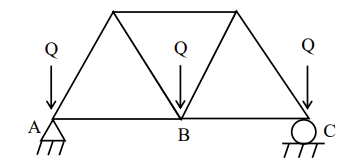
\includegraphics[width=0.5\columnwidth]{figs/ass2_d_q11.png}
    \caption{}
    \label{fig:placeholder}
\end{figure}

\begin{multicols}{2}
\begin{enumerate}
    \item 0
    \item $\dfrac{Ql}{AE}$
    \item $\dfrac{\sqrt{3}Ql}{(4AE)}$
    \item $\dfrac{Ql}{(\sqrt{3}AE)}$
\end{enumerate}
\end{multicols}
(GATE XE 2012)


\item A vertical pole, cantilevered at the bottom, has a solid circular cross-section of diameter $d=49.21~mm$. 
It is loaded by a horizontal force $P=6675~N$ at the top end. The maximum shear stress in the pole is  

\begin{multicols}{4}
\begin{enumerate}
    \item 4.25 N/mm$^2$
    \item 5.68 N/mm$^2$
    \item 4.68 N/mm$^2$
    \item 7.50 N/mm$^2$
\end{enumerate}
\end{multicols}
(GATE XE 2012)

\item A striker with mass $m=20 \,\text{kg}$ is attached to the end of a mass-less rigid bar of length $R=0.3 \,\text{m}$. The bar is hinged to support $A$, and swings down from an initial horizontal position such that the striker hits mass $M=5 \,\text{kg}$ elastically. The mass $M$ slides (in a straight line) along the table, from point $B$ towards the spring located at point $C$, $0.2 \,\text{m}$ away from $B$. Assume that the coefficient of friction in the region $BC$ is $\mu_d = 0.4$; the region $CD$ is frictionless. Let the spring constant of the spring be $k=4000 \,\text{N/m}$. If the striker rises to a maximum height of $0.1 \,\text{m}$ below its starting location, then the maximum compression of the spring is (let acceleration due to gravity $g=10 \,\text{m/s}^2$, the dimensions of the striker and mass are small)

\begin{figure}[H]
    \centering
    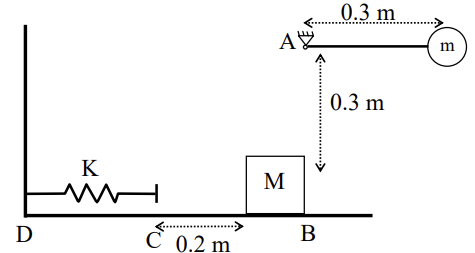
\includegraphics[width=0.5\columnwidth]{figs/ass2_d_q13.png}
    \caption{}
    \label{fig:placeholder}
\end{figure}

\begin{multicols}{4}
\begin{enumerate}
\item 0.000 m
\item 0.100 m
\item 0.089 m
\item 0.109 m
\end{enumerate}
\end{multicols}
(GATE XE 2012)

\item A cube, made of aluminum, of dimension $0.1 \,\text{m} \times 0.1 \,\text{m} \times 0.1 \,\text{m}$, rests against a rigid wall (with wall's normal in the $y$-direction), as shown in the figure. Another parallel rigid wall is located at a clearance of $0.2 \,\text{mm}$ from the block. Assuming all contacts to be frictionless, if the block is heated by $\Delta T = 150^\circ \text{C}$, the normal stress $\sigma_{yy}$ induced in the block is (for aluminum $E = 70 \,\text{GPa}; \, \nu = 0.3; \, \alpha = 20 \times 10^{-6}/^\circ \text{C}$)

\begin{figure}[H]
    \centering
    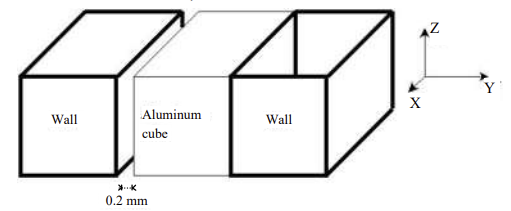
\includegraphics[width=0.5\columnwidth]{figs/ass2_d_q14.png}
    \caption{}
    \label{fig:placeholder}
\end{figure}

\begin{enumerate}
\item $\sigma_{yy} = -7 \,\text{MPa}$
\item $\sigma_{yy} = 7 \,\text{MPa}$
\item $\sigma_{yy} = -70 \,\text{MPa}$
\item $\sigma_{yy} = 0$
\end{enumerate}
(GATE XE 2012)

\item A thin walled spherical pressure vessel made of a linear elastic isotropic material has inner radius $r$ and thickness $t$ before pressurization. When subjected to internal pressure $p$, elements of the pressure vessel wall experience a state of stress described by a single point $(\sigma, \tau) = \left(\tfrac{pr}{2t},0\right)$ in Mohr's circle. The reduction of the wall thickness due to pressurization

\begin{enumerate}
\item increases with $t$
\item remains independent of $t$
\item decreases with $t$
\item depends on the elastic properties
\end{enumerate}
(GATE XE 2012)

\item For small oscillations, the natural frequency of the system in terms of $K, a, b$ and $M$ is (assuming ideal joints and mass-less rigid rod ABC)

\begin{figure}[H]
    \centering
    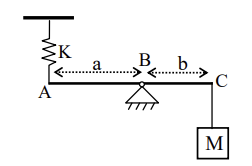
\includegraphics[width=0.5\columnwidth]{figs/ass2_d_q16.png}
    \caption{}
    \label{fig:placeholder}
\end{figure}

\begin{multicols}{4}
\begin{enumerate}
\item $\sqrt{\dfrac{K}{M}}$
\item $\sqrt{\dfrac{Ka}{Mb}}$
\item $\sqrt{\dfrac{Kb^2}{Ma^2}}$
\item $\sqrt{\dfrac{Ka^2}{Mb^2}}$
\end{enumerate}
\end{multicols}
(GATE XE 2012)

\item[] {\large \textbf{Common Data Questions}}

\textbf{Common Data for Questions 17 and 18:}

A steel cylindrical pressure vessel has an inner radius of $1.8 \, \text{m}$ and a wall thickness of $20 \, \text{mm}$. 

\item For an internal pressure of $800 \, \text{kPa}$ the maximum shear stress for the cylindrical part of the vessel is  

\begin{multicols}{4}
\begin{enumerate}
\item $16 \, \text{MPa}$
\item $18 \, \text{MPa}$
\item $20 \, \text{MPa}$
\item $0$
\end{enumerate}
\end{multicols}
(GATE XE 2012)

\item At which of the following internal pressures will the cylindrical vessel yield as per the Tresca criterion if the yield strength of the material in tension is $320 \, \text{MPa}$  

\begin{multicols}{4}
\begin{enumerate}
\item $3.55 \, \text{MPa}$
\item $7.1 \, \text{MPa}$
\item $1.775 \, \text{MPa}$
\item $4.0 \, \text{MPa}$
\end{enumerate}
\end{multicols}
(GATE XE 2012)

\item[] \textbf{Common Data for Questions 19 and 20:}

A steel beam, of rectangular cross-section $25 \, \text{mm}$ wide and $75 \, \text{mm}$ deep, is pinned to supports at points A and B, where the support B is on rollers. The Young’s modulus of steel may be assumed as $2.0 \times 10^{5} \, \text{N/mm}^2$. The ends of the beam are loaded with $5 \, \text{kN}$ loads. 

\begin{figure}[H]
    \centering
    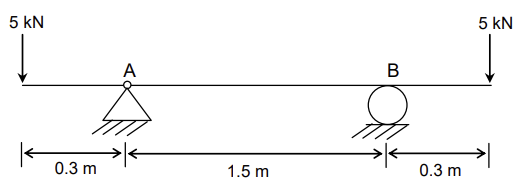
\includegraphics[width=0.5\columnwidth]{figs/ass2_d_q19.png}
    \caption{}
    \label{fig:placeholder}
\end{figure}

\item The maximum bending stress in the beam is  

\begin{multicols}{4}
\begin{enumerate}
\item $0$
\item $64 \, \text{MN/m}^2$
\item $128 \, \text{MN/m}^2$
\item $32 \, \text{MN/m}^2$
\end{enumerate}
\end{multicols}
(GATE XE 2012)

\item The vertical deflection at the ends is  

\begin{multicols}{4}
\begin{enumerate}
\item $4.92 \, \text{mm}$
\item $4.58 \, \text{mm}$
\item $9.31 \, \text{mm}$
\item $9.84 \, \text{mm}$
\end{enumerate}
\end{multicols}
(GATE XE 2012)

\item[] {\large \textbf{Linked Answer Questions}}

\textbf{Statement for Linked Answer Questions 21 and 22:}  

A cantilevered beam of unknown material (which is homogeneous, linearly elastic and isotropic) and an unknown cross-section (which is uniform and symmetric) is given in the figure. The stiffness of the end spring is $k = 2000 \, \text{N/m}$ and end load $P = 1000 \, \text{N}$; length of the beam $L = 1 \, \text{m}$. 

\begin{figure}[H]
    \centering
    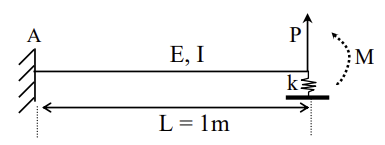
\includegraphics[width=0.5\columnwidth]{figs/ass2_d_q21.png}
    \caption{}
    \label{fig:placeholder}
\end{figure}

\item If the deflection at the free-end (under load $P$, with end moment $M=0$) is measured as $\delta = 5 \, \text{mm}$, the flexural rigidity $EI$ for the beam is (in $\text{N m}^2$)

\begin{multicols}{4}
\begin{enumerate}
\item $66,666$
\item $66,000$
\item $67,300$
\item $64,000$
\end{enumerate}
\end{multicols}
(GATE XE 2012)

\item The value of the additional end moment $M$ (in N·m) required to obtain an upward deflection of $1 \, \text{mm}$ at the free end is (moment is positive in counterclockwise direction)  

\begin{multicols}{4}
\begin{enumerate}
\item $-533.33$
\item $533.33$
\item $-528$
\item $528$
\end{enumerate}
\end{multicols}
(GATE XE 2012)


\end{enumerate}

\begin{center}
\textbf{END OF SECTION - D}
\end{center}

\newpage

\begin{center}
{\Large\textbf{E : THERMODYNAMICS}}
\end{center}



\textit{Note: Usual notations have been used for thermodynamic variables.}

\textbf{Useful Data:} \\
Unless otherwise specified, the following data may be assumed. \\
Universal gas constant, $R = 8.314 \, \text{kJ/kmol.K}$; Acceleration due to gravity, $g = 9.81 \, \text{m/s}^2$ \\
Molecular mass of air, $M_{air} = 29 \, \text{kg/kmol}$; Specific heat of air at constant pressure, $c_p = 1.005 \, \text{kJ/kg.K}$ \\
Ratio of specific heats of air, $\gamma = 1.4$. Assume air to be a perfect gas unless specified otherwise.

\begin{enumerate}

\item[] \textbf{Q.1 - Q.9 carry one mark each.}


\item Consider a piston-cylinder arrangement containing a gas. This system is heated by placing it on the top of a burner. The system undergoes  
\begin{enumerate}
    \item a constant volume process  
    \item a constant pressure process  
    \item an adiabatic process  
    \item an isothermal process  
\end{enumerate}
(GATE XE 2012)

\item For a pure substance, at the triple point  
\begin{enumerate}
    \item only solid and liquid phases co-exist in equilibrium  
    \item only liquid and vapour phases co-exist in equilibrium  
    \item only solid and vapour phases co-exist in equilibrium  
    \item solid, liquid and vapour phases co-exist in equilibrium  
\end{enumerate}
(GATE XE 2012)

\item In a saturated liquid-vapour mixture, the property quality, $x$ is defined as  
\begin{multicols}{2}
\begin{enumerate}
    \item $x = \dfrac{m_{vapour}}{m_{liquid} + m_{vapour}}$  
    \item $x = \dfrac{m_{vapour}}{m_{liquid}}$  
    \item $x = \dfrac{m_{liquid}}{m_{liquid} + m_{vapour}}$  
    \item $x = \dfrac{m_{liquid}}{m_{vapour}}$  
\end{enumerate}
\end{multicols}
(GATE XE 2012)

\item The slope of a Mollier diagram at constant pressure indicates  
\begin{multicols}{2}
\begin{enumerate}
    \item enthalpy  
    \item entropy  
    \item internal energy  
    \item temperature  
\end{enumerate}
\end{multicols}
(GATE XE 2012)

\item If $Q_L$ represents the magnitude of heat transfer from a low temperature reservoir to a cyclic device and $Q_H$ represents the magnitude of heat transfer from a cyclic device to a high temperature reservoir, then for the same $Q_L$ and $Q_H$, the coefficient performance of a refrigerator $(COP_R)$ and the coefficient performance of a heat pump $(COP_{HP})$ can be related as  
\begin{multicols}{2}
\begin{enumerate}
    \item $COP_R = 1 - COP_{HP}$  
    \item $COP_{HP} = COP_R + 1$  
    \item $COP_R \cdot COP_{HP} = 1$  
    \item $COP_{HP} = COP_R - 1$  
\end{enumerate}
\end{multicols}
(GATE XE 2012)

\item Clausius inequality is written as  
\begin{multicols}{2}
\begin{enumerate}
    \item $\oint \dfrac{\delta Q}{T} \geq 0$  
    \item $\oint \delta Q < 0$  
    \item $\oint \dfrac{\delta Q}{T} \leq 0$  
    \item $\oint \dfrac{\delta Q}{T} > 0$  
\end{enumerate}
\end{multicols}
(GATE XE 2012)

\item In a Diesel cycle, the ratio of cylinder volumes after and before combustion process is called  
\begin{multicols}{4}
\begin{enumerate}
    \item cut-off ratio  
    \item back work ratio  
    \item pressure ratio  
    \item compression ratio  
\end{enumerate}
\end{multicols}
(GATE XE 2012)

\item The exergy (or availability) of a system at a specified state  
\begin{enumerate}
    \item depends on the conditions of the system alone  
    \item depends on the conditions of the environment alone  
    \item depends on the conditions of both the system and environment  
    \item depends neither on the conditions of the system nor the environment  
\end{enumerate}
(GATE XE 2012)

\item In each of the following choices, there are two expressions given. Select the choice that gives, first, the defining expression of volume expansivity and second, the expression of volume expansivity for ideal gas  
\begin{multicols}{2}
\begin{enumerate}
    \item $\dfrac{1}{v}\left(\dfrac{\partial v}{\partial T}\right)_p, \dfrac{1}{T}$  
    \item $\dfrac{1}{v}\left(\dfrac{\partial v}{\partial P}\right)_T, \dfrac{1}{T}$  
    \item $-\dfrac{1}{v}\left(\dfrac{\partial v}{\partial P}\right)_T, \dfrac{1}{P}$  
    \item $\dfrac{1}{v}\left(\dfrac{\partial v}{\partial T}\right)_p, \dfrac{1}{P}$  
\end{enumerate}
\end{multicols}
(GATE XE 2012)

\item[] \textbf{Q.10 - Q.22 carry two marks each.}

\item A certain mass of gas at $0^{\circ}C$ is expanded to $81$ times its original volume under adiabatic conditions. If ratio of specific heats of the gas, $\gamma = 1.25$, the final temperature of the gas is  
\begin{multicols}{4}
\begin{enumerate}
    \item $-235^{\circ}C$  
    \item $-182^{\circ}C$  
    \item $-91^{\circ}C$  
    \item $0^{\circ}C$  
\end{enumerate}
\end{multicols}
(GATE XE 2012)

\item A sample of gas with initial average kinetic energy, $E$ is heated from $27^{\circ}C$ to $327^{\circ}C$. The average kinetic energy after heating is  
\begin{multicols}{4}
\begin{enumerate}
    \item $E$  
    \item $2E$  
    \item $27E$  
    \item $327E$  
\end{enumerate}
\end{multicols}
(GATE XE 2012)

\item Helium in a piston/cylinder assembly at $20^{\circ}C$ and $100 \, \text{kPa}$ is brought to $400 \, K$ in a reversible polytropic process with exponent $n = 1.25$. Assume helium to be an ideal gas. The molecular mass of helium is $4.003 \, \text{kg/kmol}$. The specific work in the process is approximately  
\begin{multicols}{4}
\begin{enumerate}
    \item $-800 \, \text{kJ/kg}$  
    \item $788 \, \text{kJ/kg}$  
    \item $788 \, \text{kJ/kg}$  
    \item $-888 \, \text{kJ/kg}$  
\end{enumerate}
\end{multicols}
(GATE XE 2012)

\item $32 \, \text{kg}$ of oxygen is mixed with $28 \, \text{kg}$ of nitrogen at the same temperature. The gases are at the same pressure of $103 \, \text{kPa}$ before and after mixing. If $\bar{R}$ is the universal gas constant in $\text{kJ/kmol.K}$, the change in entropy of the mixture is  
\begin{multicols}{4}
\begin{enumerate}
    \item $1.38\bar{R}$  
    \item $0.69\bar{R}$  
    \item $\bar{R}$  
    \item $0.34\bar{R}$  
\end{enumerate}
\end{multicols}
(GATE XE 2012)

\item Consider two Carnot heat engines A and B operating in series. Engine A receives heat from a reservoir at $1750 \, K$ and rejects heat to another reservoir at temperature $T$. Engine B receives an equal amount of energy as that rejected by Engine A from the reservoir at temperature $T$, then rejects heat to another reservoir at $320 \, K$. In both cases, the engines produce the same amount of work. If the thermal efficiencies of both the engines are the same, then the temperature $T$ is approximately  
\begin{multicols}{4}
\begin{enumerate}
    \item $848 \, K$  
    \item $748 \, K$  
    \item $648 \, K$  
    \item $548 \, K$  
\end{enumerate}
\end{multicols}
(GATE XE 2012)

\item Joule-Thomson coefficient for a gas, $\mu_{j}$ obeying the relation $p(v-b) = RT$ is
\begin{multicols}{4}
\begin{enumerate}
\item $\mu_{j} = \dfrac{c_{p}}{b}$
\item $\mu_{j} = \dfrac{b}{c_{p}}$
\item $\mu_{j} = -\dfrac{b}{c_{p}}$
\item $\mu_{j} = -\dfrac{c_{p}}{b}$
\end{enumerate}
\end{multicols}
(GATE XE 2012)

\item The correct expression representing $Z$ to be a thermodynamic property is
\begin{enumerate}
\item $Z = vdp$
\item $Z = vdp + pdv$
\item $Z = pdv + vdp$
\item $Z = pdv - vdp$
\end{enumerate}
(GATE XE 2012)

\item[] {\large \textbf{Common Data Questions}}

\textbf{Common Data for Questions 17 and 18:}

The vapour pressure of liquid ammonia (in atmosphere) in the vicinity of the triple point can be expressed as  
$$\ln p + \dfrac{3063}{T} = 15.16$$  
where temperature $T$ is expressed in K.  

In a similar manner, the vapour pressure of solid ammonia can be expressed as  
$$\ln p + \dfrac{3754}{T} = 18.7$$  

Take the molecular mass of ammonia to be 17 kg/kmol.  

\item The temperature and pressure at the triple point are
\begin{multicols}{2}
\begin{enumerate}
\item 295.2 K, 0.69 atm
\item 295.2 K, 0.59 atm
\item 195.2 K, 0.69 atm
\item 195.2 K, 0.59 atm
\end{enumerate}
\end{multicols}
(GATE XE 2012)

\item The latent heat of vaporisation is
\begin{multicols}{4}
\begin{enumerate}
\item 1298 kJ/kg
\item 1398 kJ/kg
\item 1498 kJ/kg
\item 1698 kJ/kg
\end{enumerate}
\end{multicols}
(GATE XE 2012)

\textbf{Common Data for Questions 19 and 20:}

Consider an ideal reheat cycle utilizing steam. Steam leaves the boiler and enters the turbine at 3 MPa, 400$^\circ$C (state 3) and then expands to 0.8 MPa (state 4). It is then reheated at constant pressure 0.8 MPa to 400$^\circ$C (state 5) and expands to 10 kPa in the low pressure turbine (state 6). The entry to the pump corresponds to saturated liquid state (state 1), and state 2 represents inlet to the boiler. The following data are given:

$h_{1} = 191.81 \,\text{kJ/kg}, \quad h_{3} = 323.082 \,\text{kJ/kg}, \quad h_{4} = 2891.6 \,\text{kJ/kg},$  $h_{5} = 3267.97 \,\text{kJ/kg},$

$h_{g}|_{10kPa} = 2584.63 \,\text{kJ/kg}, \quad x_{6} = 0.92285 , \quad v_{f}|_{10kPa} = 0.00101 \,\text{m}^3/\text{kg}$  

\item The heat transfer in the boiler is approximately
\begin{multicols}{2}
\begin{enumerate}
\item 4411 kJ/kg
\item 3412 kJ/kg
\item 3230 kJ/kg
\item 2892 kJ/kg
\end{enumerate}
\end{multicols}
(GATE XE 2012)

\item The net workdone in the cycle is approximately
\begin{multicols}{2}
\begin{enumerate}
\item 1004 kJ/kg
\item 1104 kJ/kg
\item 1204 kJ/kg
\item 2004 kJ/kg
\end{enumerate}
\end{multicols}
(GATE XE 2012)

\item[] {\large \textbf{Linked Answer Questions}}

\textbf{Statement for Linked Answer Questions 21 and 22:}  

A piston-cylinder arrangement as shown in the figure initially contains air at $150 \,\text{kPa}$ and $400^{\circ}\text{C}$. The arrangement is allowed to cool to the ambient temperature of $20^{\circ}\text{C}$. The characteristic gas constant for air is $0.287 \,\text{kJ/kg.K}$. The cylinder wall has stops of negligible thickness that can prevent the piston from moving down. The stops are $1 \,\text{m}$ from the inner side of the base surface of the cylinder. At the initial state, the piston is resting $1 \,\text{m}$ above the stops.

\begin{figure}[H]
    \centering
    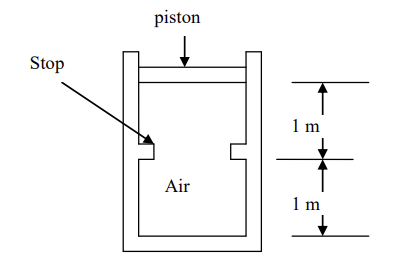
\includegraphics[width=0.5\columnwidth]{figs/ass2_e_q21.png}
    \caption{}
    \label{fig:placeholder}
\end{figure}
\item The final pressure in the cylinder is  
\begin{multicols}{2}
\begin{enumerate}
\item $130.7 \,\text{kPa}$  
\item $150 \,\text{kPa}$  
\item $200.7 \,\text{kPa}$  
\item $230.7 \,\text{kPa}$  
\end{enumerate}
\end{multicols}  
(GATE XE 2012)

\item The specific work done by the air during the process is  
\begin{multicols}{2}
\begin{enumerate}
\item $-26.67 \,\text{kJ/kg}$  
\item $26.67 \,\text{kJ/kg}$  
\item $49.5 \,\text{kJ/kg}$  
\item $-96.67 \,\text{kJ/kg}$  
\end{enumerate}
\end{multicols}  
(GATE XE 2012)



\end{enumerate}

\begin{center}
\textbf{END OF SECTION - E}
\end{center}

\newpage

\begin{center}
{\Large\textbf{F : POLYMER SCIENCE AND ENGINEERING}}
\end{center}

\begin{enumerate}

\item[] \textbf{Q.1-Q.9 carry one mark each.}

\item The diamine used for the synthesis of nylon 6,4 is
\begin{multicols}{2}
\begin{enumerate}
\item tetramethylene diamine
\item hexamethylene diamine
\item phenylene diamine
\item cyclohexane-1,4-diamine
\end{enumerate}
\end{multicols}
(GATE XE 2012)

\item A small amount of hydroquinone is added to methyl methacrylate monomer in order to
\begin{enumerate}
\item improve its thermal stability
\item improve its hydrolytic stability
\item inhibit polymerization
\item regulate molecular weight
\end{enumerate}
(GATE XE 2012)

\item Which of the following compounds is used in Ziegler–Natta catalyst?
\begin{multicols}{2}
\begin{enumerate}
\item TiCl$_3$
\item CaCl$_2$
\item ZnCl$_2$
\item NaCl
\end{enumerate}
\end{multicols}
(GATE XE 2012)

\item The z-average molecular weight, $M_z$, can be estimated using
\begin{multicols}{2}
\begin{enumerate}
\item End group analysis
\item Osmometry
\item Viscometry
\item Ultracentrifugation
\end{enumerate}
\end{multicols}
(GATE XE 2012)

\item The unit of intrinsic viscosity is
\begin{multicols}{4}
\begin{enumerate}
\item dl/g
\item g/dl
\item poise
\item g/mol
\end{enumerate}
\end{multicols}
(GATE XE 2012)

\item Heat dissipation is most inefficient in
\begin{multicols}{2}
\begin{enumerate}
\item Emulsion polymerization
\item Solution polymerization
\item Bulk polymerization
\item Suspension polymerization
\end{enumerate}
\end{multicols}
(GATE XE 2012)

\item The crystalline melting temperature of the polymers high density polyethylene (HDPE), isotactic polypropylene (iPP), nylon 6 (PA6) and poly(ethylene terephthalate) (PET) can be arranged as
\begin{multicols}{2}
\begin{enumerate}
\item $T_{HDPE} > T_{PET} > T_{iPP} > T_{PA6}$
\item $T_{PET} > T_{PA6} > T_{iPP} > T_{HDPE}$
\item $T_{PA6} > T_{HDPE} > T_{PET} > T_{iPP}$
\item $T_{iPP} > T_{PA6} > T_{PET} > T_{HDPE}$
\end{enumerate}
\end{multicols}
(GATE XE 2012)

\item Which of the following polymers is sensitive to moisture absorption?
\begin{multicols}{4}
\begin{enumerate}
\item Polyethylene
\item Polystyrene
\item Polyamide 6
\item Polybutadiene
\end{enumerate}
\end{multicols}
(GATE XE 2012)

\item Most engineering polymers have heat distortion temperature (HDT) in excess of
\begin{multicols}{4}
\begin{enumerate}
\item $-80^\circ$C
\item $0^\circ$C
\item $20^\circ$C
\item $80^\circ$C
\end{enumerate}
\end{multicols}
(GATE XE 2012)

\item[] \textbf{Q.10-Q.22 carry two marks each}

\item Two miscible polymers A and B are blended in weight ratio of 30:70. If the glass transition temperature, $T_g$, of polymer A is $-50^\circ$C and that of polymer B is $100^\circ$C, then the $T_g$ of the blend is
\begin{multicols}{4}
\begin{enumerate}
\item $-10.5^\circ$C
\item $25.0^\circ$C
\item $37.5^\circ$C
\item $74.8^\circ$C
\end{enumerate}
\end{multicols}
(GATE XE 2012)


\item If the flow curves of two viscous fluids are represented by

\begin{figure}[H]
    \centering
    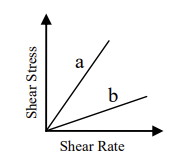
\includegraphics[width=0.5\columnwidth]{figs/ass2_f_q11.png}
    \caption{}
    \label{fig:placeholder}
\end{figure}

then, the viscosity plots of the fluids will be
\begin{multicols}{2}
\begin{enumerate}
\item \begin{figure}[H]
    \centering
    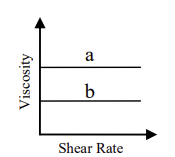
\includegraphics[width=0.5\columnwidth]{figs/ass2_f_q11_a.png}
    \caption{}
    \label{fig:placeholder}
\end{figure}
\item\begin{figure}[H]
    \centering
    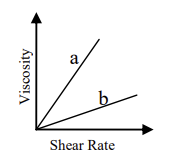
\includegraphics[width=0.5\columnwidth]{figs/ass2_f_q11_b.png}
    \caption{}
    \label{fig:placeholder}
\end{figure}
\item \begin{figure}[H]
    \centering
    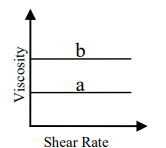
\includegraphics[width=0.5\columnwidth]{figs/ass2_f_q11_c.png}
    \caption{}
    \label{fig:placeholder}
\end{figure}
\item \begin{figure}[H]
    \centering
    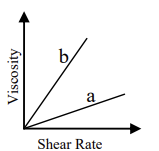
\includegraphics[width=0.5\columnwidth]{figs/ass2_f_q11_d.png}
    \caption{}
    \label{fig:placeholder}
\end{figure}
\end{enumerate}
\end{multicols}
(GATE XE 2012)

\item Match the following compounding ingredients in plastic technology with their respective functions:

\begin{table}[H]
\centering
\begin{tabular}{l l}
Compounding ingredients & Functions \\
P. Tricresyl phosphate & 1. Filler \\
Q. Calcium carbonate & 2. UV stabilizer \\
R. Azodicarbonamide & 3. Plasticizer \\
S. o-Hydroxybenzophenone & 4. Blowing agent \\
\hline
\end{tabular}
\caption{}
\label{}
\end{table}

\begin{multicols}{2}
\begin{enumerate}
\item P-3, Q-1, R-4, S-2
\item P-1, Q-4, R-3, S-2
\item P-4, Q-1, R-2, S-3
\item P-3, Q-4, R-1, S-2
\end{enumerate}
\end{multicols}
(GATE XE 2012)

\item In a three-point bending mode for flexural test of a polymer sample with the following data:  

\begin{center}
load applied in the mid-span $= 80$ kg  

width of the specimen $= 3$ cm  

depth of the specimen $= 2$ cm 

length of the specimen $= 30$ cm  
\end{center}

the flexural strength will be
\begin{multicols}{4}
\begin{enumerate}
\item 17.5 MPa
\item 29.4 MPa
\item 35.7 MPa
\item 41.3 MPa
\end{enumerate}
\end{multicols}
(GATE XE 2012)

\item How many stereo isomers are possible in total on polymerization of butadiene?
\begin{multicols}{4}
\begin{enumerate}
\item 2
\item 3
\item 4
\item 5
\end{enumerate}
\end{multicols}
(GATE XE 2012)

\item Match the following processing operations with their respective tools:  

\begin{table}[H]
\centering
\begin{tabular}{ll}
\textbf{Processing operations} & \textbf{Tools} \\
P. Injection molding & 1. Parison mold \\
Q. Twin screw extrusion & 2. Sprue-runner system \\
R. Blow molding & 3. Mixing head \\
S. Reaction injection molding & 4. Kneading blocks \\
\end{tabular}
\caption{}
\label{}
\end{table}

\begin{multicols}{2}
\begin{enumerate}
\item P-1, Q-2, R-3, S-4
\item P-2, Q-4, R-1, S-3
\item P-2, Q-1, R-4, S-3
\item P-4, Q-1, R-2, S-3
\end{enumerate}
\end{multicols}
(GATE XE 2012)

\item If a solid elastomer ball of weight $100 \, \text{g}$ is allowed to free fall from a height of $10 \, \text{m}$ and it rebounds back to a height of $8 \, \text{m}$, the hysteresis loss is  

\begin{multicols}{4}
\begin{enumerate}
\item 19.60 J
\item 9.80 J
\item 1.96 J
\item 0.98 J
\end{enumerate}
\end{multicols}
(GATE XE 2012)


\item[]  {\large \textbf{Common Data Questions}  }

\noindent \textbf{Common Data for Questions 17 and 18:}  

A polymer mixture contains three monodisperse polystyrene samples A, B and C of molecular weights $10000$, $20000$ and $30000 \, \text{g mol}^{-1}$, respectively.  


\item If the mixture contains equal number of molecules of A, B and C, the weight average molecular weight, $M_w$ will be  

\begin{multicols}{2}
\begin{enumerate}
\item $1.93 \times 10^4 \, \text{g mol}^{-1}$
\item $2.13 \times 10^4 \, \text{g mol}^{-1}$
\item $2.33 \times 10^4 \, \text{g mol}^{-1}$
\item $2.53 \times 10^4 \, \text{g mol}^{-1}$
\end{enumerate}
\end{multicols}
(GATE XE 2012)

\item If the mixture contains equal masses of A, B and C, then the number average molecular weight, $M_n$ will be  

\begin{multicols}{2}
\begin{enumerate}
\item $1.64 \times 10^4 \, \text{g mol}^{-1}$
\item $1.74 \times 10^4 \, \text{g mol}^{-1}$
\item $1.84 \times 10^4 \, \text{g mol}^{-1}$
\item $1.94 \times 10^4 \, \text{g mol}^{-1}$
\end{enumerate}
\end{multicols}
(GATE XE 2012)



\item[] \textbf{Common Data for Questions 19 and 20:}  

The stress relaxation equation for polymers is given by, $\sigma = \sigma_0 e^{-t/\tau}$, where $\sigma$ is the stress at any time instant $t$, $\sigma_0$ is the initial stress and $\tau$ is the relaxation time. The relaxation process is temperature dependent and follows the Arrhenius law. For a rubber sample, the relaxation time is $60$ days at $25^{\circ}\text{C}$.  


\item If the above sample is stressed to $2 \, \text{MPa}$ initially, then the time required to relax the stress to $1 \, \text{MPa}$ will be  

\begin{multicols}{2}
\begin{enumerate}
\item 31.6 days
\item 41.6 days
\item 51.6 days
\item 61.6 days
\end{enumerate}
\end{multicols}
(GATE XE 2012)

\item If the activation energy for relaxation is $30 \, \text{kJ mol}^{-1}$, the relaxation time at $35^{\circ}\text{C}$ will be  

\begin{multicols}{2}
\begin{enumerate}
\item 30.5 days
\item 35.5 days
\item 40.5 days
\item 45.5 days
\end{enumerate}
\end{multicols}
(GATE XE 2012)

\item[] {\large \textbf{Linked Answer Questions}} 

\textbf{Statement for Linked Answer Questions 21 and 22:} 

In tensile testing of carbon fiber reinforced epoxy composite samples, the following data were recorded: 
\begin{center}
gauge length = 4 cm 

cross-section = 0.8 cm $\times$ 0.3 cm 

increase in gauge length at the break point = 0.03 cm 

breaking load = 50 kg 
\end{center}

  \item Considering the stress-strain curve to be linear up to the break point, the tensile strength is
  \begin{multicols}{2}
  \begin{enumerate}
    \item 191.2 kg/cm$^2$
    \item 208.3 kg/cm$^2$
    \item 312.1 kg/cm$^2$
    \item 535.5 kg/cm$^2$
  \end{enumerate}
  \end{multicols}
  (GATE XE 2012)

  \item The Young’s modulus of the composite is
  \begin{multicols}{2}
  \begin{enumerate}
    \item 1.77 $\times$ 10$^4$ kg/cm$^2$
    \item 1.99 $\times$ 10$^4$ kg/cm$^2$
    \item 2.34 $\times$ 10$^4$ kg/cm$^2$
    \item 2.77 $\times$ 10$^4$ kg/cm$^2$
  \end{enumerate}
  \end{multicols}
  (GATE XE 2012)

\end{enumerate}

\begin{center}
\textbf{END OF SECTION - F}
\end{center}

\newpage

\begin{center}
{\Large\textbf{G : FOOD TECHNOLOGY}}
\end{center}

\begin{enumerate}

\item[] \textbf{Q.1-Q.9 carry one mark each.}

  \item Among the following fatty acids, which group is known as essential fatty acids?
  \begin{enumerate}
    \item 9,11-Octadecadienoic and 9,11,13-Octadecatrienoic
    \item 9,12-Octadecadienoic and 9,12,15-Octadecatrienoic
    \item 9-Octadecenoic and 9,11-Octadecadienoic
    \item 9,11-Octadecadienoic and 9-Eicosenoic
  \end{enumerate}
  (GATE XE 2012)

  \item Cellulose, the structural polysaccharide of plant, is a polymer of
  \begin{enumerate}
    \item $\beta$-D-Glucose
    \item $\alpha$-D-Glucose
    \item $\beta$-D-Galactose
    \item $\alpha$-D-Galacturonic acid
  \end{enumerate}
  (GATE XE 2012)

  \item The important role of carotenoids in the human diet is their ability to serve as precursors of
  \begin{multicols}{4}
  \begin{enumerate}
    \item Vitamin C
    \item Vitamin D
    \item Vitamin A
    \item Vitamin K
  \end{enumerate}
  \end{multicols}
  (GATE XE 2012)

  \item Which one of the following microorganisms is used in the preparation of bread?
  \begin{multicols}{2}
  \begin{enumerate}
    \item \textit{Candida utilis}
    \item \textit{Saccharomyces cerevisiae}
    \item \textit{Saccharomyces cerevarum}
    \item \textit{Aspergillus niger}
  \end{enumerate}
  \end{multicols}
  (GATE XE 2012)

  \item Which one of the microorganisms given below is NOT RESPONSIBLE for ropy or stringy fermentation of milk?
  \begin{enumerate}
    \item \textit{Alcaligenes viscolactis}
    \item \textit{Enterobacter aerogenes}
    \item \textit{Streptococcus cremoris}
    \item \textit{Streptococcus lactis}
  \end{enumerate}
  (GATE XE 2012)

  \item A mild heat treatment of foods that destroys pathogens and extends its shelf life is called
  \begin{multicols}{2}
  \begin{enumerate}
    \item Baking
    \item Blanching
    \item Sterilization
    \item Pasteurization
  \end{enumerate}
  \end{multicols}
  (GATE XE 2012)

  \item The most common and least expensive plastic film used for packaging of solid food materials is
  \begin{multicols}{2}
  \begin{enumerate}
    \item Polyethylene
    \item Polystyrene
    \item Polypropylene
    \item Polyvinylchloride
  \end{enumerate}
  \end{multicols}
  (GATE XE 2012)

  \item Reassociation of amylose and formation of crystalline structure upon cooling of cooked starch solution is termed as
  \begin{multicols}{2}
  \begin{enumerate}
    \item Syneresis
    \item Gelatinization
    \item Retrogradation
    \item Denaturation
  \end{enumerate}
  \end{multicols}
  (GATE XE 2012)

  \item Thermal destruction of microorganisms follows a kinetics of
  \begin{enumerate}
    \item Zero order
    \item First order
    \item Second order
    \item Fractional order
  \end{enumerate}
  (GATE XE 2012)

\item[] \textbf{Q.10-Q.22 carry two marks each.}

  \item Which one of the following is NOT A CORRECT statement?
\begin{enumerate}
    \item Meatiness is the taste produced by compounds such as glutamate in products like cheese, soy sauce. 
    \item Astringency is a dry mouth feel in the oral cavity that is most associated with phenolic compounds. 
    \item Saltiness is a taste that is mainly produced by chloride ions. 
    \item Sourness is related to acidity and is sensed by hydrogen ion channels in the human tongue.
\end{enumerate}
(GATE XE 2012)

\item The following plot represents the \textit{Lineweaver-Burk} equation of an enzymatic reaction both in the presence and the absence of inhibitor. Here, $V$ is the velocity of reaction and $S$ is the substrate concentration.  

\begin{figure}[H]
    \centering
    \caption{} \label{}
    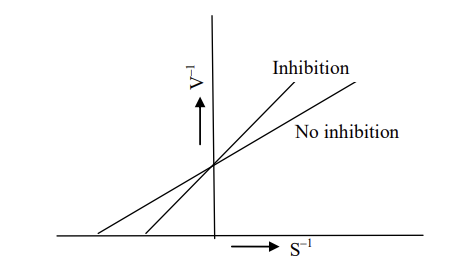
\includegraphics[width=0.5\columnwidth]{figs/ass2_g_q11.png}
    \caption{}
    \label{fig:placeholder}
\end{figure}

The nature of inhibition shown in the plot is
\begin{enumerate}
    \item Non-competitive
    \item Anti-competitive
    \item Competitive
    \item Mixed type
\end{enumerate}
(GATE XE 2012)

\item Make the correct match of the food constituents in \textbf{Group I} with their nature given in \textbf{Group II}.  

\begin{table}[H]
\centering
\caption{} \label{}
\begin{tabular}{l l}
Group I & Group II \\
Ascorbic Acid & Antioxidant \\
Phenyl alanine & Amino Acid \\
Dextrose & Sugar \\
Haemoglobin & Chelate \\
\hline
\end{tabular}
\end{table}

\begin{multicols}{2}
\begin{enumerate}
    \item P-4, Q-3, R-1, S-2  
    \item P-4, Q-1, R-3, S-2  
    \item P-3, Q-4, R-2, S-1  
    \item P-4, Q-2, R-1, S-3  
\end{enumerate}
\end{multicols}
(GATE XE 2012)

\item Make the correct match of the fermented food products in \textbf{Group I} with the microorganisms in \textbf{Group II}.  

\begin{table}[H]
\centering
\begin{tabular}{l l}
Group I & Group II \\
Yoghurt & \textit{Lactobacillus acidophilus}, \textit{Lactobacillus delbrueckii} \\
Cheese & \textit{Leuconostoc mesenteroides}, \textit{Lactobacillus plantarum} \\
Sauerkraut & \textit{Lactobacillus delbrueckii}, \textit{Streptococcus thermophilus} \\
Kefir & \textit{Lactobacillus casei}, \textit{Streptococcus thermophilus} \\
\hline
\end{tabular}
\end{table}

\begin{multicols}{2}
\begin{enumerate}
    \item P-1, Q-4, R-2, S-3  
    \item P-4, Q-3, R-1, S-2  
    \item P-3, Q-4, R-2, S-1  
    \item P-3, Q-2, R-4, S-1  
\end{enumerate}
\end{multicols}
(GATE XE 2012)

\item Match the following between organelle or cellular components of a bacterium cell in Group I with the constituents and functionalities in Group II.  

\begin{table}[H]
\centering
\caption{} \label{}
\begin{tabular}{l l}
\textbf{Group I} & \textbf{Group II} \\
P) Cytoplasmic membrane & 1) Protein synthesis \\
Q) Flagellum & 2) Peptidoglycan \\
R) Cell wall & 3) Phospholipid bilayer \\
S) Ribosome & 4) Motility of cell \\
\end{tabular}
\end{table}

\begin{multicols}{4}
\begin{enumerate}
\item P-3, Q-2, R-4, S-1  
\item P-4, Q-2, R-1, S-3  
\item P-3, Q-4, R-2, S-1  
\item P-2, Q-3, R-4, S-1  
\end{enumerate}
\end{multicols}
(GATE XE 2012)

\item Thermal death time (TDT) of \textit{Clostridium botulinum} at $121^{\circ}$C is $2.78 \, \text{min}$ with a $z$-value of $10^{\circ}$C.  
The TDT of the microorganism at $116^{\circ}$C (in min) is  

\begin{multicols}{4}
\begin{enumerate}
\item 5.270  
\item 8.791  
\item 1.390  
\item 0.712  
\end{enumerate}
\end{multicols}
(GATE XE 2012)

\item Make the correct match between specific food processing operations in Group I with their mechanism of action in Group II.  

\begin{table}[H]
\centering
\caption{} \label{}
\begin{tabular}{l l}
\textbf{Group I} & \textbf{Group II} \\
P) Ball Mill & 1) Compression and shear \\
Q) Roller Mill & 2) Pressure bursting \\
R) Flash Peeling & 3) Friction and shear \\
S) Abrasive Peeling & 4) Impact and shear \\
\end{tabular}
\end{table}

\begin{multicols}{2}
\begin{enumerate}
\item P-4, Q-2, R-1, S-3  
\item P-4, Q-1, R-2, S-3  
\item P-4, Q-3, R-2, S-1  
\item P-3, Q-1, R-4, S-2  
\end{enumerate}
\end{multicols}
(GATE XE 2012)

\item[] {\large \textbf{Common Data Questions}}

\textbf{Common Data for Questions 17 and 18:}

650 g of a wet food containing 405 g water is dried in a tray dryer to a final moisture content of $6.8 \, \%$ (dry basis). It is observed that the drying process occurs under constant rate period and it takes $8 \, \text{h}$.

\item Initial moisture content (in percentage) of the food on wet basis is  

\begin{multicols}{4}
\begin{enumerate}
\item 62.31  
\item 70.45  
\item 162.31  
\item 165.31  
\end{enumerate}
\end{multicols}

\item The rate of drying (in kg/h) is  

\begin{multicols}{4}
\begin{enumerate}
\item 128.79  
\item 126.35  
\item 77.81  
\item 0.0485  
\end{enumerate}
\end{multicols}
(GATE XE 2012)

\item[] \textbf{Common Data for Questions 19 and 20:}

Air at 1 atmospheric pressure (101.325 kPa) and $30^\circ$C with absolute humidity of 0.0218 kg/kg of dry air is flowing in a drying chamber. The saturated vapor pressure of water ($p_{w}^{\text{sat}}$, in kPa) is related to temperature ($T$, in $^\circ$C) as given below

$$
\ln p_{w}^{\text{sat}} = 18.6556 - \frac{5217.635}{T+273}
$$

Heat capacities of dry air (average molecular weight 29) and that of water vapor (molecular weight 18) are 1.005 and 1.884 kJ/kg.K, respectively. Latent heat of vaporization of water at reference temperature (0 $^\circ$C) is 2502.3 kJ/kg.

\item The relative humidity of air (in percentage) is 

\begin{multicols}{4}
\begin{enumerate}
\item 62.82
\item 68.22
\item 86.62
\item 81.80
\end{enumerate}
\end{multicols}
(GATE XE 2012)

\item The enthalpy (in kJ/kg) of moist air is

\begin{multicols}{4}
\begin{enumerate}
\item 85.93
\item 54.55
\item 31.38
\item 99.38
\end{enumerate}
\end{multicols}
(GATE XE 2012)



\item[]  {\large \textbf{Linked Answer Questions}}

\textbf{Statement for Linked Answer Questions 21 and 22: }

 The total solids content in a milk sample is 18\%. It is desired to produce 1000 kg of sweetened condensed milk (SCM) having 40\% sugar, 25\% moisture and rest milk solids.

\item What is the ‘Sugar Ratio’ (in percentage) in the SCM in terms of sugar and water content in the final product?

\begin{multicols}{4}
\begin{enumerate}
\item 48.19
\item 61.54
\item 54.16
\item 56.14
\end{enumerate}
\end{multicols}
(GATE XE 2012)

\item If the ‘Concentration Degree’ is 2.5, the amount of sugar added in kg in the milk sample is

\begin{multicols}{4}
\begin{enumerate}
\item 246.16
\item 216.64
\item 192.76
\item 224.56
\end{enumerate}
\end{multicols}
(GATE XE 2012)


\end{enumerate}

\begin{center}
    {\Large \textbf{END OF QUESTION PAPER}}
\end{center}
\end{document}
